\section{Task-Support Temporal Analysis}
\label{appx:task_support}

\subsection{Implementation Fact}

The task-support channel is the slice $\mathrm{relation\_adj}[:,2,:,:]$ (receiver--sender orientation). An edge is active only when the receiver--sender pair is role-compatible, the corresponding communication edge is available, and the sender currently holds task-relevant information (target information or a local attack window). Task-Support is therefore a task-dependent relational mask over delivered communication; it is not an independent communication channel and does not decide whether real messages are sent.

\subsection{Window Statistics}

Table~\ref{tab:s1_ts_windows} and Fig.~\ref{fig:s2_windows} report the locked window statistics of the Full method (9 blue--blue pairs; 3 training seeds; windows fixed to $[-20,-1]$, $[0,20]$, $[r-20,r-1]$, $[r,r+20]$ relative to failure step $f$ and recovery step $r$). The pre-failure window shows the highest activation ($0.141$), and activation \emph{decreases} in the early post-failure window ($0.092$; pooled difference $-0.0488$, with all three seeds showing the same downward direction). The pre-recovery window ($0.090$) shows no rebound ($\mathrm{pre\text{-}rec} - \mathrm{early} \approx 0$). These results do not support a post-failure activation increase or relational-restructuring hypothesis.

A data fact worth stating explicitly: in this evaluation, recovery coincides with episode termination in all $952/952$ recovered episodes (recovery step equals the final step). The post-recovery window is therefore undefined; the pre-recovery window is the effective tail window. This is a property of the evaluation protocol, not missing data.

\begin{figure}[t]
    \centering
    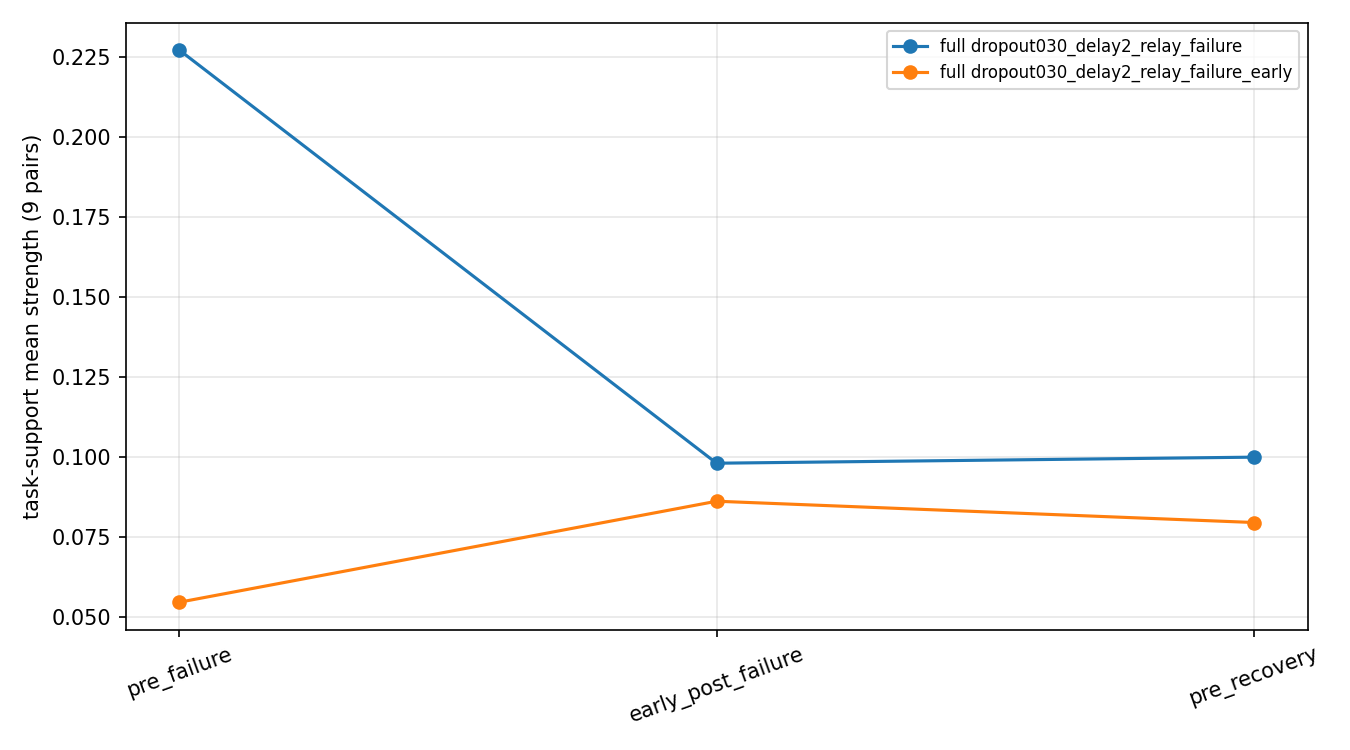
\includegraphics[width=0.85\linewidth]{figures/fig_task_support_windows.png}
    \caption{Task-Support relation strength by window (Full, pooled over episodes). 
    Activation decreases after failure and does not rebound before recovery.}
    \label{fig:s2_windows}
\end{figure}

\begin{table}[t]
\centering
\small
\caption{Task-Support relation strength by window (9 blue--blue pairs; 3 training seeds; pooled over episodes). Early-post and pre-recovery are lower than pre-failure; no post-failure activation increase.
\label{tab:s1_ts_windows}
\begin{tabular}{lcccc}
\toprule
Window & Full pooled & seed0 & seed1 & seed2 \\
\midrule
pre_failure & 0.1409 & 0.1333 & 0.1417 & 0.1476 \\
early_post_failure & 0.0920 & 0.0923 & 0.0911 & 0.0927 \\
pre_recovery & 0.0900 & 0.0909 & 0.0877 & 0.0913 \\
\midrule
early$_\text{post}$ $-$ pre & $-0.0488$ & down & down & down \\
pre-rec $-$ early & $\approx 0$ & \multicolumn{3}{c}{no rebound} \\
\bottomrule
\end{tabular}
\end{table}

\subsection{Recovered vs.\ Failed Episodes}

Table~\ref{tab:s1_ts_windows} (main text) reports the performance ablation; here we contrast Full episodes that recover with those that do not. The first support-activation step after failure is similar ($32.96$ recovered vs.\ $32.23$ failed), the unique active role-pair count is identical ($2.996$ vs.\ $3.000$), and support persistence is longer in failed episodes ($4.74$ vs.\ $8.80$; consistent with longer failed trajectories). None of these contrasts shows a strong, consistent separation between recovery outcomes. We therefore interpret the Task-Support contribution as \textbf{empirical support only}: removing it degrades held-out recovery and slows recovery (main text RQ3), but the internal temporal pattern does not reveal a consistent post-failure restructuring mechanism.

\subsection{Case Examples (Pre-registered Selection)}

Fig.~\ref{fig:s2_cases} and Table~\ref{tab:s2_cases} show the three case classes defined by the pre-registered rule (smallest episode index within each class, evaluated with Full seed 0, scenario \texttt{dropout030\_delay2\_relay\_failure}): C1 both methods succeed but Full recovers faster; C2 Full succeeds while w/o Task-Support fails; C3 both fail. Cases were selected by this fixed rule, not by manual choice.

\begin{figure}[t]
    \centering
    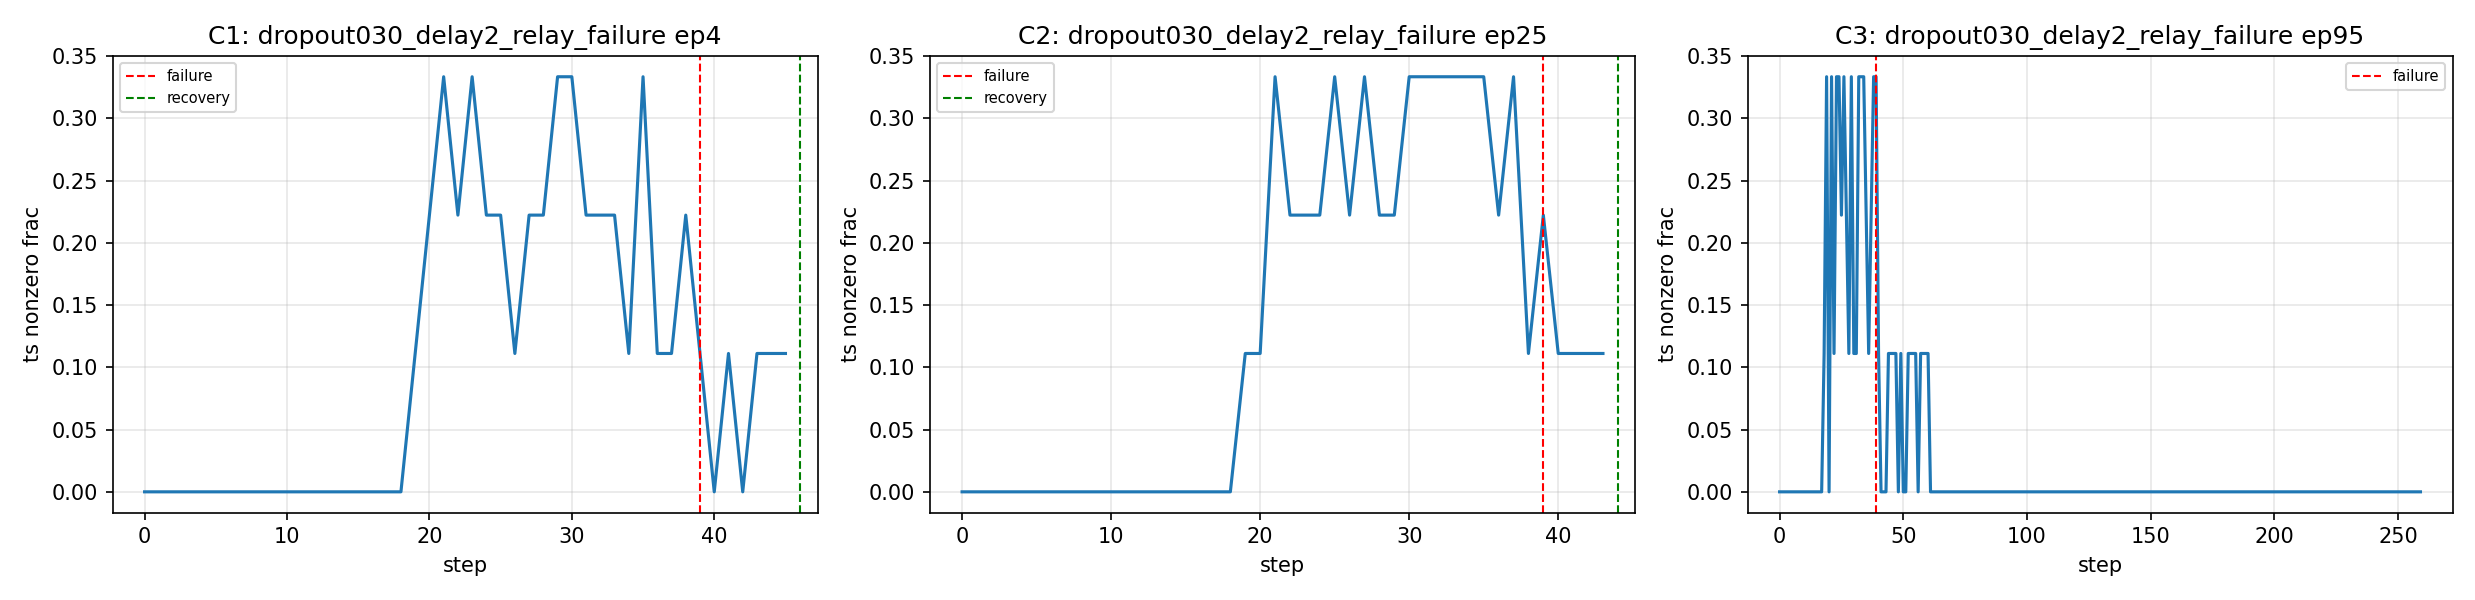
\includegraphics[width=0.95\linewidth]{figures/fig_task_support_cases.png}
    \caption{Task-Support case examples selected by the pre-registered rule (C1/C2/C3; 
    failure step in red, recovery step in green).}
    \label{fig:s2_cases}
\end{figure}

\begin{table}[t]
\centering
\small
\caption{Case examples selected by the pre-registered rule (smallest episode index within each class), not by manual choice. C1: both succeed, Full recovers faster; C2: Full succeeds, w/o Task-Support fails; C3: both fail.
\label{tab:s2_cases}
\begin{tabular}{lllrrrr}
\toprule
Class & Scenario & Ep. & Full succ. & Fail step & Full rec. & w/o-TS rec. \\
\midrule
C1 & dropout030_delay2_relay_failure & 4 & 1 & 39 & 46 & 49 \\
C2 & dropout030_delay2_relay_failure & 25 & 1 & 39 & 44 & -1 \\
C3 & dropout030_delay2_relay_failure & 95 & 0 & 39 & -1 & -1 \\
\bottomrule
\end{tabular}
\end{table}
